\chapter{Methods}

\section{Classical Computer Vision-based Approach}

This section is related to all the experiments done on the classical computer 
vision-based approach. The general scheme of the driver's attention model is 
shown in Figure \ref{fig:driver_attention}. 
The model is divided into four main stages: data synchronization, homography 
projection of the gaze, scene perception, and the driver's behavioral model. 

The data synchronization stage is responsible for aligning the data from the 
different sensors. In particular it is important that gaze data and 
images from the 
eye-tracking glasses are well synchronized each other and with video frames 
from the camera installed on the roof top of the car.

The homography projection of the gaze stage is responsible for projecting the 
gaze of the driver from the ETG camera plane to the roof top camera plane.
In this way we have a wider, more stable and accurate representation of 
the outside environment.
It is possible to 
estimate the homography transformation making the approximation that the matched 
keypoints are far away enough from the vehicle. This is a reasonable 
approximation since the driver is usually looking at the road and the objects 
far away from the vehicle. Moreover, the baseline of the stereo vision system is 
small compared to the depth of the keypoints.
The optimal way to estimate the projection would be through the epipolar 
geometry, estimating the fundamental matrix and the essential matrix. 
However, we have an uncalibrated stereo setup, and the baseline between the two 
cameras is not fixed. Even though it could be possible to integrate GPS data 
to estimate the two matrices, there is a consistent noise error that affects 
accuracy of the estimation.
The homography estimation is then divided in three steps: detection of keypoints 
in the two images through the SIFT algorithm, matching of the keypoints through 
RANSAC, and estimation of the homography matrix through the least squares method.

The scene perception stage is responsible for detecting and tracking the vulnerable 
users in the scene, such as pedestrians and cyclists. The detection is done 
through the YOLOv8 algorithm and the tracking through ByteTrack. In this way 
it is possible to compare the gaze of the driver with the state of the targets, 
including their position.

Finally, on the top, there is the driver's attention model. The responsibility 
of this block is to classify dangerous scenarios given the data from the 
driver and the scene. However, this block is sensitive to the quality of the 
signals of the previous stages.

\begin{figure}
    \centering
    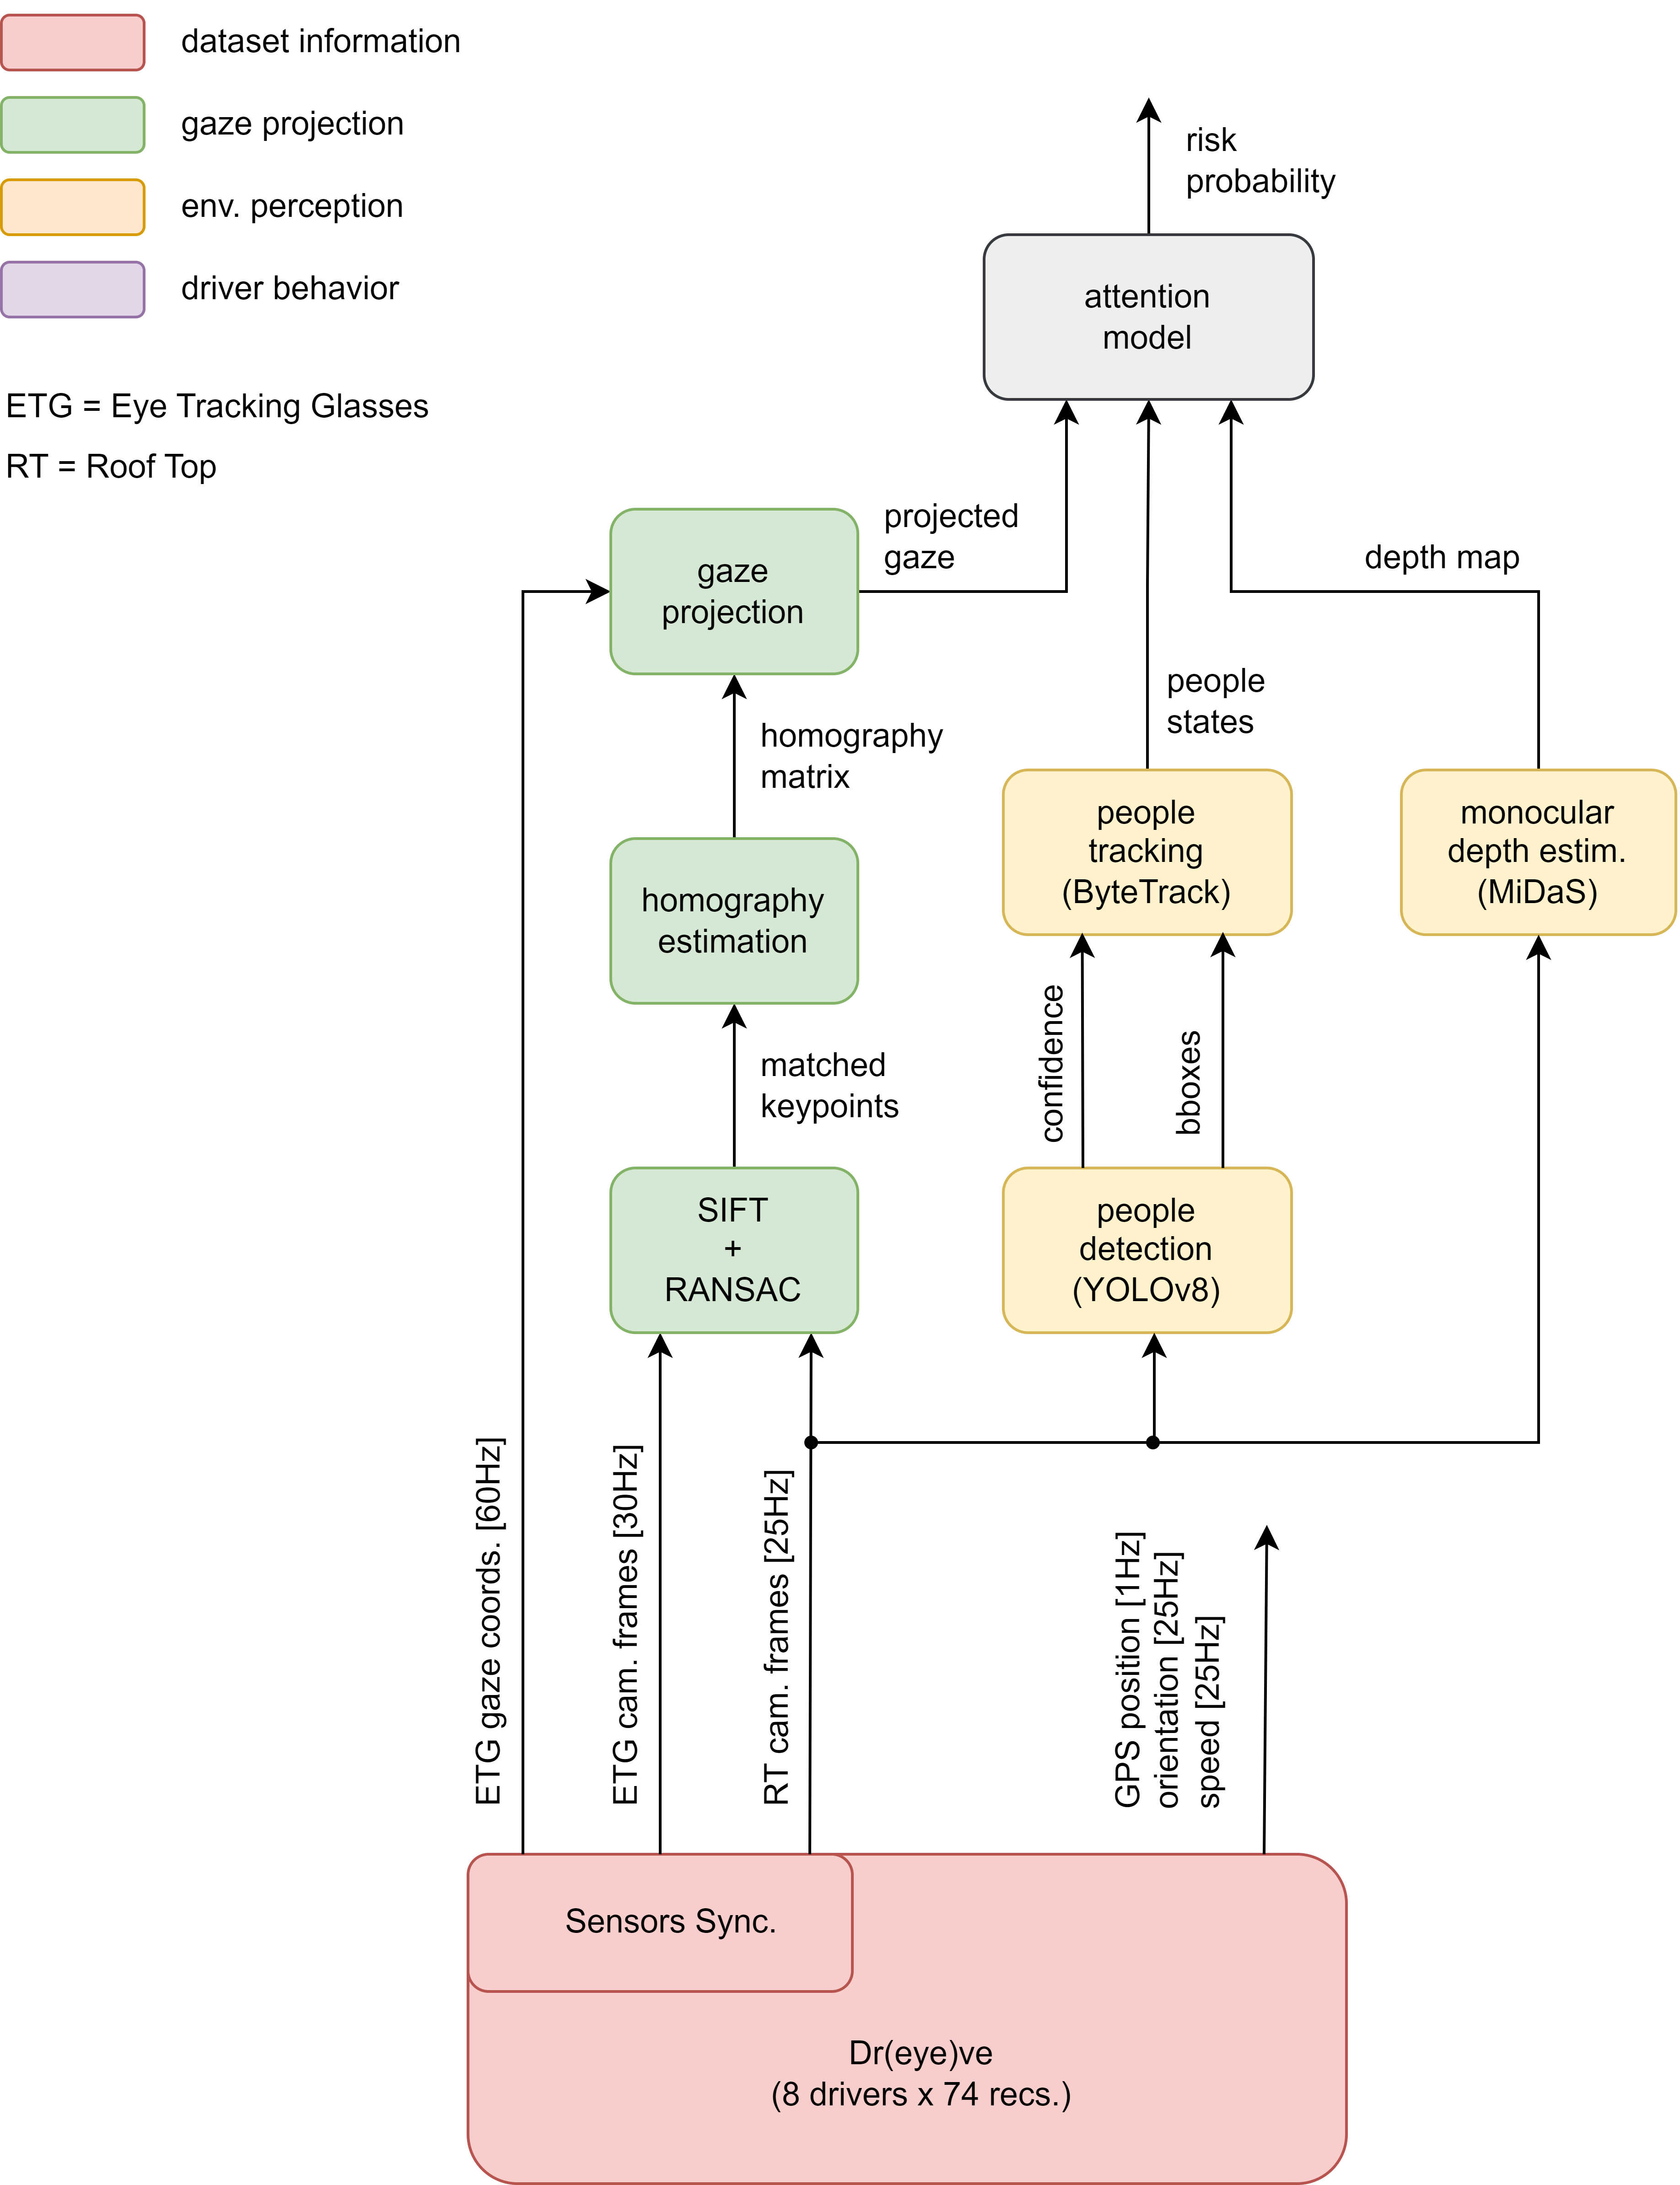
\includegraphics[width=0.9\textwidth]{images/dreyeve/classic_scheme.png}
    \vspace*{0.6cm}
    \caption{The overall driver's attention scheme. It is divided into four main 
    stages: data synchronization, homography projection of the gaze, scene 
    perception and the driver's behavioral model.
    }
    \label{fig:driver_attention}
\end{figure}

\subsection{Homography Data Preprocessing}
The Dr(eye)ve dataset is composed of 74 sequences of five minutes each. 
Moreover, the two cameras are not synchronized. 
The ETG camera has a frame rate of 30 fps, while the roof top camera has a 
frame rate of 25 fps. It is also important to notice that there are some videos 
that was recorded at slightly different frame rates. All the synchronization data 
are provided in the dataset.

Therefore, we decided to implement 
an interface to preprocess all the frames and synchronize them.
After the synchronization, we compute all the homographies and store them in a 
file. This file is then used to project the gaze of the driver in the roof top 
camera plane.
Furthermore, we chose to store other informations related to the quality of the 
estimation.
The data structure is described in Figure \ref{fig:homography_data_structure}:
it is a list of lists where each element is a unique sample that has the 
following fields: the gaze coordinates in the ETG and RT camera planes, the 
homography matrix, detected keypoints on the two planes, and the number of 
matchings between them.

\begin{figure}
    \centering
    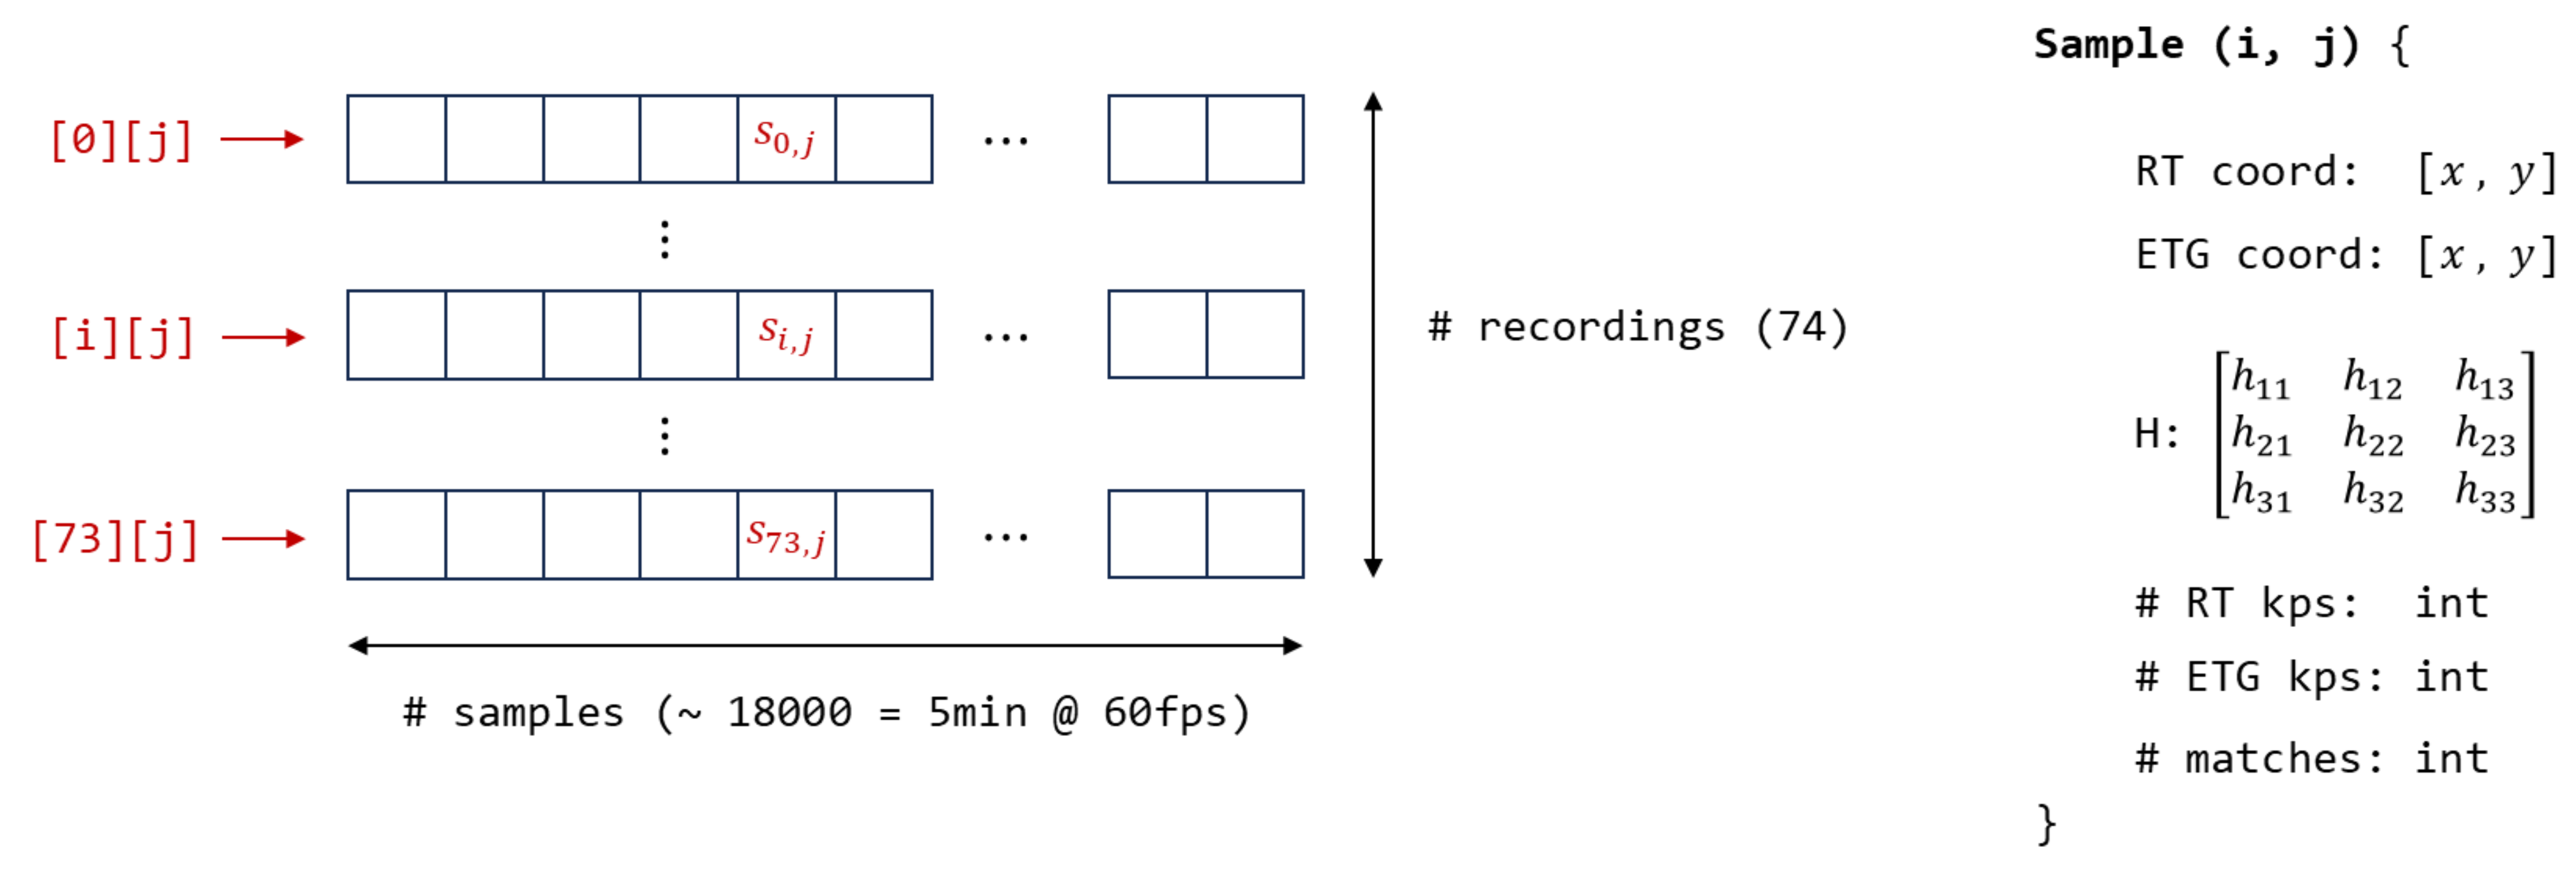
\includegraphics[width=\textwidth]{images/dreyeve/homography_data.png}
    \caption{The data structure used to store the homographies.
    \textbf{Left}: Each element is a specific sample in the i-th video, at 
    the j-th frame.
    \textbf{Right}: The attributes of each sample.}
    \label{fig:homography_data_structure}
\end{figure}

\subsection{Stereo Camera System Setup}
The cameras recording setup can be reconducted to an uncalibrated stereo vision 
setup. In particular, the two cameras are not aligned and the baseline is not 
fixed. However, this is a problem for the projection of 3D world points between 
the two cameras. In fact, the homography matrix is a planar transformation, 
and it is not able to project points that are not on the same plane of the 
keypoints. For this reason we decided to make the approximation that the 
keypoints are far away enough from the vehicle. This is a reasonable 
approximation since the driver is usually looking at the road and the objects 
far away from the vehicle. Moreover, the baseline of the stereo vision system is 
small compared to the average depth of the keypoints.


\subsection{Targets Data Structure}



\section{Deep Learning-based Approach}

\subsection{Attention Mechanism for Dangerous Scene Detection}

\subsection{The Artificial Bias}

\subsection{Data Preprocessing of Dr(eye)ve}

\subsection{Data Preprocessing of BDD100k}


\subsection{Handling Unbalanced Data}

\subsubsection{Evaluation Metrics}

\subsubsection{Data Augmentation}

% \subsubsection{Upsampling}

% \subsubsection{Downsampling}	

\subsubsection{Weighting Loss Function}

% \subsubsection{Synthetic Minority Oversampling Technique (SMOTE)}

% \subsection{Receiver Operating Characteristic (ROC) Curve}